\documentclass[10pt,a4paper]{article}
\usepackage[margin=0.72in]{geometry}
\usepackage{fontspec}
\setmainfont{TeX Gyre Termes}
\setsansfont{TeX Gyre Heros}
\setmonofont{Latin Modern Mono}[Scale=0.85]
\usepackage{amsmath,booktabs,tabularx,graphicx,xcolor,microtype}
\usepackage{unicode-math}
\setmathfont{TeX Gyre Termes Math}
\usepackage[font=small,labelfont=bf]{caption}
\usepackage[numbers,sort&compress]{natbib}
\usepackage[colorlinks=true,linkcolor=teal,citecolor=teal,urlcolor=teal]{hyperref}
\usepackage{fancyhdr}
\pagestyle{fancy}
\fancyhf{}
\fancyhead[L]{\small SGMem: speaker- and group-aware memory}
\fancyhead[R]{\small AIAA 4051 | Topic 12}
\fancyfoot[L]{\footnotesize Team-review draft | 23 November 2026}
\fancyfoot[R]{\thepage}
\setlength{\headheight}{14pt}
\setlength{\parindent}{1em}
\setlength{\parskip}{2pt}
\setlength{\textfloatsep}{10pt}
\setlength{\floatsep}{8pt}
\setlength{\abovecaptionskip}{5pt}
\setlength{\belowcaptionskip}{2pt}
\newcommand{\TestRows}{%
Multi-hop & 137 & 27.74 & 24.82 & 26.28 & 27.74 \\
Knowledge update & 80 & 32.50 & 20.00 & 31.25 & 32.50 \\
Temporal & 122 & 22.95 & 12.30 & 18.03 & 19.67 \\
User-implicit & 36 & 33.33 & 36.11 & 36.11 & 33.33 \\
Term ambiguity & 79 & 13.92 & 20.25 & 17.72 & 25.32 \\
Abstention & 82 & 76.83 & 63.41 & 65.85 & 69.51 \\
\textbf{Overall} & 536 & 33.21 & 27.24 & 30.60 & 33.02 \\
}
\newcommand{\DevRows}{%
Fields & 55 & 30.73 & 0.461 \\
Scope & 62 & 34.64 & 0.457 \\
Person & 64 & 35.75 & 0.461 \\
Time & 62 & 34.64 & 0.439 \\
Hybrid & 62 & 34.64 & 0.486 \\
Hybrid-meta & 65 & 36.31 & 0.575 \\
Scope+reply & 62 & 34.64 & 0.882 \\
Focus & 63 & 35.20 & 0.882 \\
}
\newcommand{\CostRows}{%
Full BM25/Dense baseline & 3.5907 \\
Bounded-reply dev & 0.4303 \\
Ordered-reply dev & 0.4376 \\
Metadata exploration and frozen test & 8.7841 \\
Additional recorded pilots and smoke tests & 0.1063 \\
\textbf{Recorded subtotal (incomplete history)} & 13.3489 \\
}

\title{\vspace{-1.3em}\textbf{When Metadata Helps Multi-Party Memory:}\\A Controlled Study with Local Language Models\vspace{-0.4em}}
\author{SGMem course project | AIAA 4051, Topic 12}
\date{23 November 2026\vspace{-0.8em}}

\begin{document}
\fontsize{10.5}{12.7}\selectfont
\maketitle
\thispagestyle{fancy}
\begin{abstract}
Multi-party memory must preserve the association between content, speakers, groups and evolving decisions. We study a small, training-free metadata retrieval change on GroupMemBench using local Qwen3-8B and E5-small-v2. First, we reproduce the released BM25 and dense retrieval workflow on all 715 questions. We then diagnose 38 failed baseline records from 24 development questions, with 61 checked source messages. A focused modification adds a public-metadata candidate list to lexical and dense rank fusion. Eight configurations are evaluated on 179 fixed development questions before selecting and freezing the final method. On 536 held-out questions, metadata improves hybrid retrieval from 164 to 177 correct answers: 35 gains and 22 losses, or +2.43 percentage points. This difference is not statistically significant under a question-level paired test ($p=0.111$), and the result remains one answer below BM25. Source-grounded cases show both recovered evidence and harmful displacement. The study supports a limited structural benefit rather than a general accuracy improvement, and documents generation costs, judge disagreements and reproducibility boundaries.
\end{abstract}

\section{Problem and research context}
A message can be relevant in wording while belonging to the wrong project, speaker or decision stage. For example, two Health IT Specialists may discuss different field maps; retrieving either message without resolving the project can produce a plausible but incorrect answer. Our question is whether \emph{public conversational metadata used during retrieval} improves answers over content-only memory under a fixed local QA setup.

Retrieval-augmented generation combines retrieved external information with a language model \cite{rag}. GroupMemBench extends the evaluation setting to synthetic multi-party conversations with six question types and asker identities \cite{groupmembench}. Its content baselines expose speaker and role information to QA after retrieval. We instead test whether structured information should influence which memories reach QA. Graph-based memory systems such as HippoRAG use knowledge graphs and Personalized PageRank \cite{hipporag}; our course study asks how far a small metadata branch can go without building such a system.

We use E5 contrastive embeddings \cite{e5} and Qwen3 \cite{qwen3} as local, fixed components. Reciprocal rank fusion (RRF) is an established unsupervised combination rule \cite{rrf}; it is not our proposed algorithmic novelty. Our contribution is a controlled investigation of a metadata candidate branch, its connection to observed group-memory failures, and the conditions under which it helps or harms a local-model baseline.

\section{Reproduction and evaluation protocol}
\paragraph{Data and split.}
We pin the official GroupMemBench repository to commit \texttt{461f00c}. Each of Finance, Technology, Healthcare and Manufacturing contains 30,000 messages; their question counts are 214, 213, 130 and 158. A seed-42, domain/category-stratified split fixes 179 development and 536 test questions. Both partitions share the same domain histories, so this is held-out-question evaluation, not generalization to unseen conversations. Released questions have no query timestamp; we follow the upstream full-domain history visibility instead of deriving a cutoff from an answer.

\paragraph{Baselines and model control.}
BM25 uses the upstream content tokenization and stable ordering. E5-small-v2 uses \texttt{query:}/\texttt{passage:} prefixes, normalized 384-dimensional embeddings and exact cosine search, with its 512-token encoder limit \cite{e5card}. Both return ten original messages with the same metadata formatting. We verified BM25 IDs, order and scores against the upstream implementation for all 715 questions, and checked QA/judge formatting and parsing against the official code. Dense is an open-source embedding substitution, not an exact reproduction of the original commercial embedding model.

All methods share Qwen3-8B (revision \texttt{b968826}) for answering and judging, BF16/SDPA, non-thinking mode, temperature 0.2, top-$p$ 1, top-$k$ 0, seed 42 per call, and answer/judge limits of 512/256 output tokens. Embedding-based methods share E5 revision \texttt{ffb93f3}. Reference answers enter only the judge and post-hoc analysis. Retrieval receives the public question and asker identity. Formal runs use Transformers 4.57.1 and PyTorch 2.8.0+cu128; a separate HTTP/Docker setup is not the source of these scores.

The full baseline results are BM25 234/715 (32.73\%) and Dense 204/715 (28.53\%). There are 1,430 completed records and 2,860 model calls, with no call errors or unclear judgments. Answer truncations are 5 and 10; neither judge truncated. Full-715 category results are in \texttt{docs/part12-full-results.md}. Comparisons below use the same 536 test IDs for every method.

\section{Failure analysis and a focused repair}
\subsection{Source-grounded diagnosis}
We inspect a fixed development quota sample of 24 questions across domains and categories, yielding 48 paired answers and 38 judged failures. Each failed record has a primary label, optional additional labels, an error stage, and source-message evidence. Labels were produced by AI-assisted source review; they are not independently human-adjudicated gold labels. The 61 checked messages make the explanations auditable, but the small quota sample is not a prevalence estimate for all failures.

\begin{figure}[htbp]
\centering
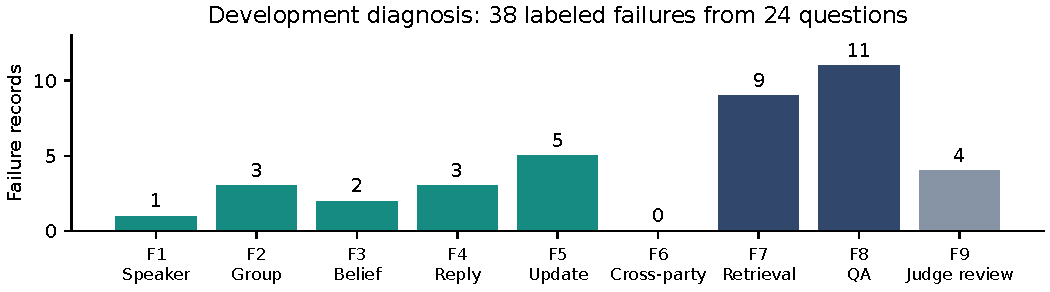
\includegraphics[width=\linewidth]{figures/failure-taxonomy.pdf}
\caption{Primary labels in the diagnostic sample. F1--F6 concern conversation structure; F7 and F8 separate other retrieval and QA failures. F9 contains four evaluation disagreements and does not change official scores. F6 has zero primary cases in this sample, not evidence that cross-participant failures never occur.}
\label{fig:taxonomy}
\end{figure}

Fourteen records have a structural primary label; nine are other retrieval failures, eleven are QA failures and four require judge review (Figure~\ref{fig:taxonomy}). By stage, 14 are retrieval, 12 QA, eight mixed and four evaluation. These are different classifications, not competing totals. Among 28 failed records with identified positive support, the baseline top ten contains support in six. Adding all two-hop reply neighbors reaches ten, but expands the diagnostic pool beyond $K=10$; this is reachability, not an equal-budget QA gain.

Two cases motivate selective metadata. In Healthcare \texttt{multi\_hop\_48}, baseline outputs confuse a Nurse Leader with the requested Health IT Specialist or use another project's EHR mapping. In \texttt{knowledge\_update\_5}, a response mixes field operations from other groups instead of the Hand Hygiene plan. Conversely, some temporal questions already retrieve the correct timestamp but still receive the wrong answer. A retrieval change cannot be assumed to repair failures of reading or judgment.

\subsection{Metadata candidate retrieval}
Each message retains its original content plus speaker, role, group, phase, topic, time and reply-to fields. We build a catalog of public names, normalize case and punctuation, and match complete names in the question. Longer names suppress contained shorter matches at the same position, while explicitly distinct matches remain. The residual content query removes matched names to reduce repeated project-name dominance.

The optional metadata list searches messages in the matched scope and, when supported, an explicitly targeted speaker or role. First-person conditions require a personal-state cue; the asker is not automatically the target. When scope and actor constraints are both available they are intersected; otherwise the available constraint is used. Candidates must have a positive residual BM25 score. If there is no usable metadata branch, the original content branches remain. This rule is conservative and does not resolve arbitrary pronouns or implicit social relationships.

Let $R$ be the available ranked lists and $r_j(m)$ a message's one-based rank in list $j$. We use
\begin{equation}
s(m)=\sum_{j\in R:m\in j}\frac{1}{60+r_j(m)}.
\label{eq:rrf}
\end{equation}
\textbf{Hybrid} combines BM25 and E5. \textbf{Hybrid-meta} adds the metadata-constrained lexical list. Each list has up to 50 candidates; ties use the original message index. Both select ten original messages for QA. The branch addition changes internal candidate computation: hybrid has at most 100 unique candidates and hybrid-meta at most 150 (observed dev maximum 145). Thus the controlled endpoint is the same final context budget, not identical internal search effort or pure reranking of an identical pool.

For $L$ lists of depth $d$ and $C$ unique candidates, fusion and sorting cost $O(Ld+C\log C)$. This excludes corpus scoring, embedding and full-list sorting in the existing retrievers. No model is trained, and no LLM is called to route a query or rerank candidates.

\section{Development comparisons and frozen test}
\subsection{Selection and ablations}
Eight prespecified configurations share the same implementation: field-augmented BM25, scope retrieval, scope plus person, conditional recency, content hybrid, hybrid-meta, bounded reply expansion, and a main-question branch. Reply expansion protects the first eight messages and can replace at most two using bounded same-group neighbors; the focus branch only triggers on recognized background clauses. These are diagnostic alternatives, not eight components of the final model.

\begin{table}[htbp]
\centering\small
\caption{Full development comparison, 179 questions per row. GPU-hours measure the individual QA run including model/index setup and judging. Retrieval preflight and outer launch overhead are accounted separately.}
\label{tab:dev}
\begin{tabular}{lrrr}\toprule
Configuration & Correct & Accuracy (\%) & GPU-hours \\\midrule
\DevRows
\bottomrule\end{tabular}
\end{table}

BM25 and Dense development controls score 56/179 and 58/179. Selection includes seven new metadata variants plus two earlier reply variants (56/179 and 57/179); content-only hybrid is a control. Hybrid-meta wins the predeclared correctness criterion with 65/179 (Table~\ref{tab:dev}), without a tie-break. The freeze was written on 21 November 2026 at 20:11:20 UTC, before either frozen hybrid test run; archived BM25/Dense tests predate it. Selection after eight new configurations can be optimistic, so final conclusions use the frozen test.

The simpler person-versus-scope comparison gains two answers without losses. Adding conditional recency loses two, and adding bounded replies changes evidence but gains no correct answers over scope. The focus rule gains one answer and triggers on only one development question. These results do not justify deeper reply graphs or more hand-written triggers. In the biased support diagnostic subset, hybrid-meta has a target in the final ten for 11/18 questions versus 8/18 for hybrid. This is not benchmark-wide recall and does not by itself establish QA improvement.

\subsection{Held-out results}
Both frozen arms complete all 536 test questions. Hybrid-meta answers 177 correctly, compared with 164 for hybrid, 178 for BM25 and 146 for Dense. There are 142 questions both hybrid arms answer correctly, 337 both miss, 35 gains and 22 losses. The net improvement is 13/536, or 2.43 percentage points. An exact, two-sided McNemar test gives $p=0.111$; questions share histories and families, further limiting independence assumptions. We do not claim statistically established superiority over hybrid or any improvement over BM25.

\begin{figure}[htbp]
\centering
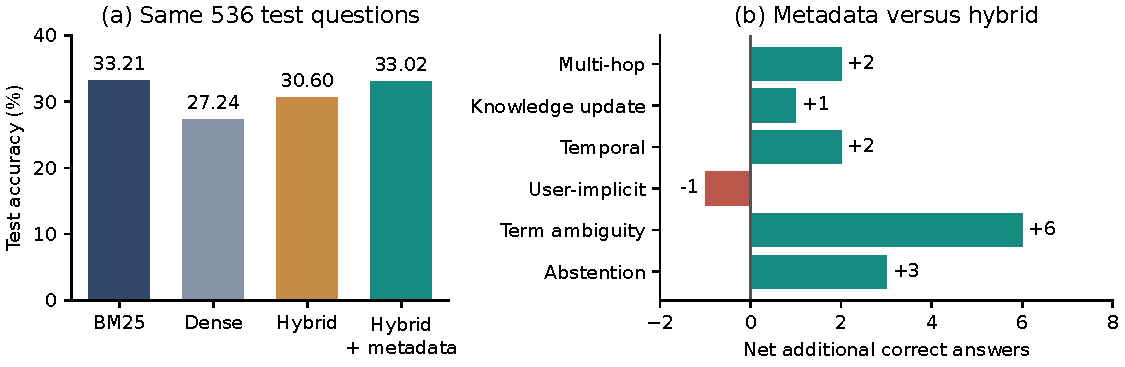
\includegraphics[width=\linewidth]{figures/test-results.pdf}
\caption{Frozen test outcomes. Metadata recovers some losses of content fusion, but the best overall baseline remains BM25. Category changes are net question counts relative to hybrid, not rates of speaker/group errors.}
\label{fig:test}
\end{figure}

\begin{table}[htbp]
\centering\small
\caption{Accuracy (\%) on the same fixed test questions. Hybrid-meta's term-ambiguity improvement does not eliminate losses relative to BM25 on temporal reasoning and abstention.}
\label{tab:test}
\begin{tabular}{lrrrrr}\toprule
Category & $n$ & BM25 & Dense & Hybrid & Hybrid-meta \\\midrule
\TestRows
\bottomrule\end{tabular}
\end{table}

Term ambiguity improves from 14/79 to 20/79 over hybrid (Table~\ref{tab:test}). Relative to BM25, its gain of nine is offset by four fewer temporal answers and six fewer abstention answers, with the other three totals unchanged. The net hybrid-meta gains by domain are Finance +7, Manufacturing +8, Technology $-1$ and Healthcare $-1$. Benefits therefore do not hold uniformly across domains or question types.

\section{Mechanisms, failures and judgment limits}
\paragraph{A role-linked repair (development).}
For Healthcare \texttt{multi\_hop\_48}, person-aware retrieval moves \texttt{Msg\_24002} from outside scope's top ten to rank 3, changing the answer to the correct action: validate and freeze the demand-forecasting field map. Hybrid-meta places it fourth and likewise repairs hybrid's EHR-mapping answer. The recognized role is the target of the question, not the asker's identity. This connects a Part 2 attribution failure to an actual metadata-triggered retrieval change.

\paragraph{New support and displaced support (test).}
For Technology \texttt{multi\_hop\_24}, \texttt{Msg\_27529} newly enters at rank 5 and supplies the mismatch exception lane, named owner and last-approved schema-hash; the answer changes from abstention to correct. In \texttt{term\_ambiguity\_30}, however, metadata displaces rank-10 \texttt{Msg\_1010}, which specifies five to ten QA edge cases. A previously correct answer becomes abstention. These examples show the value and cost of the same additional branch, not independent causal estimates for each feature.

\paragraph{Support is not sufficient.}
For Healthcare \texttt{temporal\_23}, the correct deadline message remains rank 1 under both arms, yet the metadata answer abstains. Another date in the added context may interfere, but we did not isolate this cause experimentally. Finance \texttt{multi\_hop\_1} receives exactly the same context in both arms and both select a policy-freeze date rather than the requested validation deadline. These cases locate important limitations downstream of evidence retrieval.

\paragraph{Judge disagreement.}
For Finance \texttt{term\_ambiguity\_14}, both answers express July 29 against a reference of 2025-07-29. The judge accepts hybrid's sentence but rejects the metadata answer for missing year/format, although the question does not explicitly request ISO formatting. We preserve both original labels. This is evidence of possible evaluation noise, not grounds to manually increase a score or estimate its population error rate. A teammate review of the four development F9 records and selected test disagreements remains advisable; it is not presented as already completed.

\clearpage
\section{Computational efficiency and reproducibility}
\paragraph{Measurement and trade-offs.}
Experiments run on single visible NVIDIA RTX A6000 GPUs; baseline Dense was split over two workers with disjoint questions. GPU-hours sum process residence on each GPU, including loading, indexing and judging; they are not utilization integrals. Baseline mean retrieval/answer/judge times are 0.114/5.227/2.988 seconds for BM25 and 0.013/6.187/3.329 seconds for Dense. Faster dense lookup does not imply lower end-to-end cost, since generation dominates. Two Dense workers each built an index, and this duplication is included.

\begin{figure}[htbp]
\centering
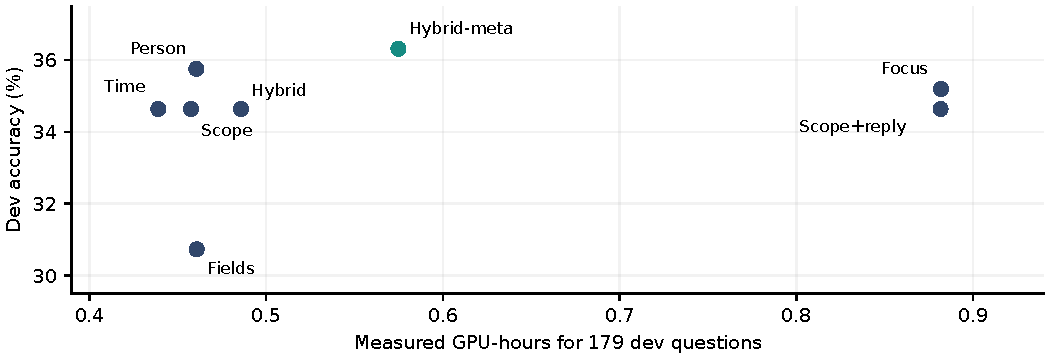
\includegraphics[width=.9\linewidth]{figures/dev-cost.pdf}
\caption{Quality versus measured run cost on 179 development questions. This is not an algorithmic efficiency frontier: device time slots and generation throughput differ. Scope+reply and focus have similar retrieval times to scope, but slower observed generation.}
\label{fig:cost}
\end{figure}

Hybrid-meta test consumes 2.1964 GPU-hours, with 94,343 answer and 53,245 judge output tokens and a 15.95 GiB peak PyTorch allocation. Hybrid consumes 1.7502 GPU-hours including the interruption, with 537 answer calls (one repeated after interruption) and 536 judge calls. Its complete first-session CPU time, index time and GPU peak were not saved; its measured resume peak is 15.90 GiB, not a whole-run maximum. The two arms' generation rates differ (about 19.2 versus 24.6 tokens/s), so GPU-hour differences cannot be attributed solely to the metadata branch.

\begin{table}[htbp]
\centering\small
\caption{Non-overlapping costs from surviving timing receipts. This subtotal excludes unmetered historical work; two additional reply preflights are documented only as approximately 0.0065 and 0.0040 GPU-hours.}
\label{tab:budget}
\begin{tabular}{lr}\toprule
Experiment scope & GPU-hours \\\midrule
\CostRows
\bottomrule\end{tabular}
\end{table}

The metadata round uses 8.7841 GPU-hours including preflight, development, test and interruption. The initial budget stopped hybrid after 246 complete questions; the authorized continuation finished only the remaining 290. Outer ledgers are counted once, not added again to nested run totals (Table~\ref{tab:budget}). Missing older connectivity timings prevent a precise whole-project total. No new generation was used to create this report or demonstration.

\paragraph{Reproducibility evidence.}
The frozen generation/retrieval commit is \texttt{3cbf1db}; later audit changes do not alter its protocol. The repository retains split, selection, runtime and per-question evidence. CPU checks reconstruct all 10,720 final retrieved passages and 2,144 answer/judge prompts with the fixed tokenizer. All 269 unchanged paired contexts have identical answers and labels, and the 246 completed pre-interruption results were not regenerated. The frozen report can be recomputed from raw records; the pre-report CPU suite passed 119 tests. The accompanying HTML demonstration replays six stored cases and clearly distinguishes replay from live inference.

\clearpage
\section{Limitations and conclusion}
The evidence is restricted to one synthetic benchmark, shared-dialogue question splits, one local QA/judge model, one generation seed and a small, nonrandom, AI-assisted failure sample. Public phase/topic labels may be cleaner than metadata in real conversations. Metadata increases the candidate pool; we do not isolate its semantic benefit from all search-budget effects. Automated judgment and answer truncation remain imperfect (five metadata and six hybrid test answers reach the limit; no judge does).

Within these boundaries, the project completes baseline reproduction, structural diagnosis and a focused metadata modification. It finds recoverable speaker/group mistakes and an observed gain over content fusion, alongside no overall gain over BM25. The useful outcome is an auditable account of when metadata changes the right evidence and when QA or displaced content becomes the bottleneck. The present evidence favors stopping additional heuristic exploration and improving communication and independent case review.

\bibliographystyle{unsrt}
\bibliography{references}
\end{document}
